\section{Implementations}
	\paragraph{}
	All our implementations (Server, Android client and iOS client) are available on GitHub (\url{https://github.com/quentinlesceller/Puzzlr}) under MIT License.
	\subsection{Server side}
 		\subsubsection{Requirements}
 		 	\paragraph{}
 			For this implementations, we were looking for a decentralized and secure open source server. The server should have some kind of API in order to easily develop with. The idea of a blockchain based server was a natural choice as Bitcoin and others cryptocurrencies can provide a very reliable decentralized ledger.
 			\subsubsection{Fabric} 
 			\paragraph{}
 			\textbf{What is Fabric ?}
 			\begin{displayquote}The Fabric is ledger of digital events, called transactions, shared among different participants, each having a stake in the system. The ledger can only be updated by consensus of the participants, and, once recorded, information can never be altered. Each recorded event is cryptographically verifiable with proof of agreement from the participants.
 			\paragraph{}
 			Transactions are secured, private, and confidential. Each participant registers with proof of identity to the network membership services to gain access to the system. Transactions are issued with derived certificates unlinkable to the individual participant, offering a complete anonymity on the network. Transaction content is encrypted with sophisticated key derivation functions to ensure only intended participants may see the content, protecting the confidentiality of the business transactions.
 			\paragraph{}
 			The fabric is an implementation of blockchain technology, where Bitcoin could be a simple application built on the fabric. It is a modular architecture allowing components to be plug-and-play by implementing this protocol specification. It features powerful container technology to host any main stream language for smart contracts development. Leveraging familiar and proven technologies is the motto of the fabric architecture.
 			\end{displayquote}
 			\paragraph{}
 			Fabric was released in December 2015\footnote{See \url{https://github.com/openblockchain}, now moved at  \url{https://github.com/hyperledger/}} and is part of the Linux's Foundation Hyperledger Project\footnote{See \url{https://www.hyperledger.org/}} which is a ``collaborative effort created to advance blockchain technology by identifying and addressing important features for a cross-industry open standard for distributed ledgers that can transform the way business transactions are conducted globally.''
 			\paragraph{}
			Fabric is written mostly in Go and a REST API is implemented.
			
			 \begin{figure}[H]
	    		 \centering
	     		 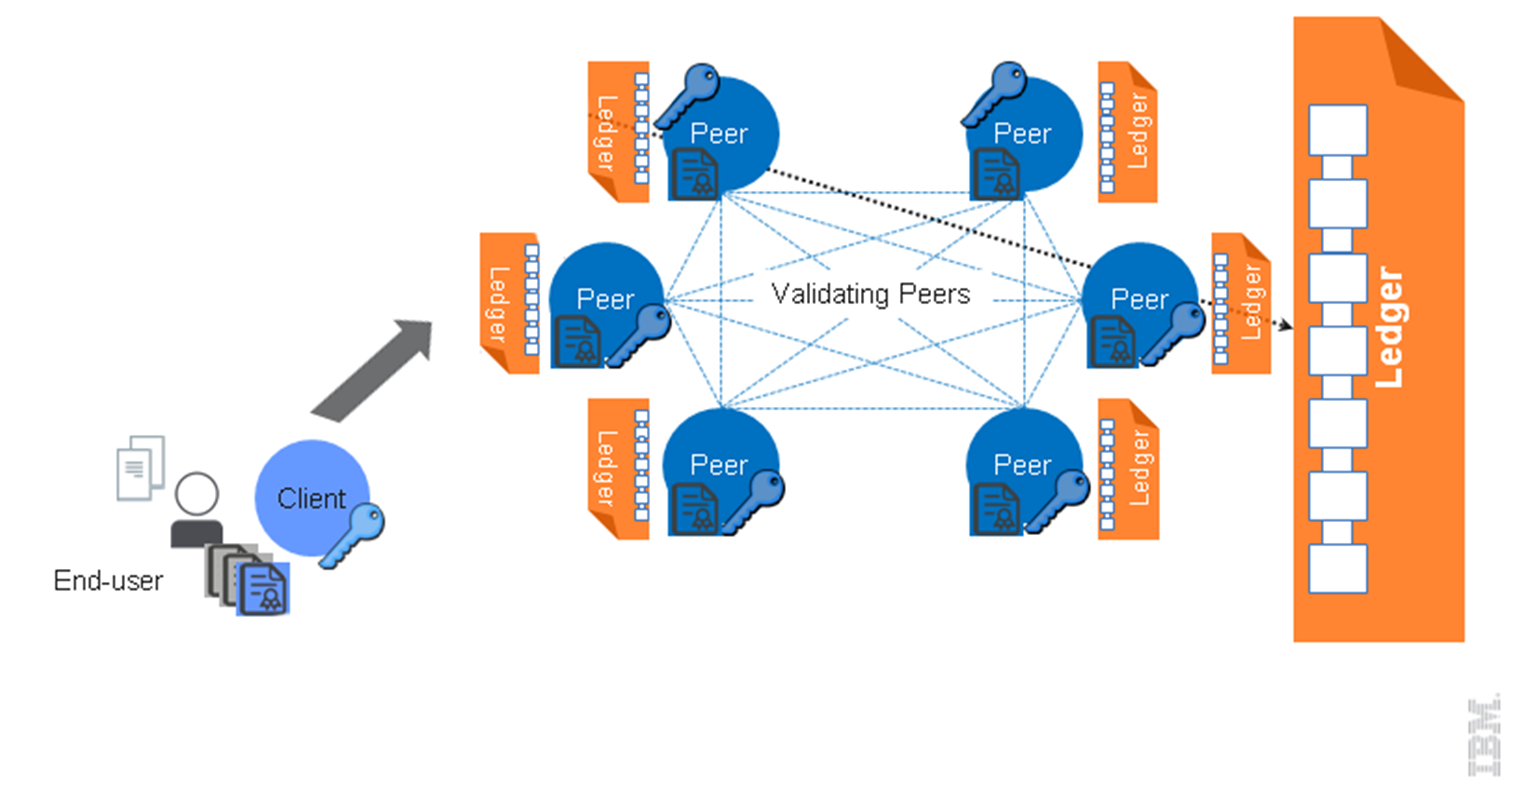
\includegraphics[width=14cm]{images/Fabric/Fabric}
	     		 \caption{Fabric Overview}
	   		\end{figure}
			
			 \textbf{Why use Fabric ?}
			 \paragraph{}
			 Building our server over the Fabric allowed us to build an unstoppable application.\\An App that run exactly as programmed without any possibility of downtime, censorship, fraud or third party interference.\\
			 
			  \textbf{How we worked with Fabric}
			   \paragraph{}
			 For our application to work, we used 3 tables (aka Chaincodes) : 
 			\begin{itemize}
 			\item User, store username and hashed password.
 			\item Key, store the public keys.
 			\item Data, store the data.
 			\end{itemize}
 			This tables are written in Go and available on the Github of the project. We will not review here the code but we can highlight that these chaincodes were developped with security in mind (e.g: the ledger will not reveal if it was the username or the password that was wrong in order to avoid user enumerations).
 			\paragraph{}
 			We released Fabric4J\footnote{Available at \url{https://github.com/quentinlesceller/Fabric4J}} the first Java API for Fabric. There is also a Swift equivalent embedded in the iOS app but we do not plan to release it at this time (as it is less complete and was just created for the purpose of being used in Puzzlr).
 	\subsection{Client side}
 		\subsubsection{Android}
  			\paragraph{}
			The Android version is written in Java Programming Language alongside with some parts in XML (the Graphical User Interface). In this project we used Android Studio as an Integrated Development Environment (IDE). The application is compatible with almost all versions of Android.
	  	
	\subsubsection{IOS}
	\paragraph{}
	We also wrote an iOS version of Puzzlr. This version was written in Swift and was challenging because Swift is a relatively new language and we had to use a lot of different frameworks and modify them in order to have a working application. The code is made to be readable with a lot of comment and comprehensive variables.
	We used 6 frameworks and forked 4 of them.

	\begin{table}[H]
	\centering
	\begin{tabular}{|c|c|c|c|c|}
  	\hline
  	Name  & Author & License & Forked & Usage \\
  	\hline
  	AsymmetricCryptoManager & Ignacio Nieto Carvajal & MIT & Y &  RSA Keys Generation\\
  	CryptoSwift & Marcin Krzyżanowski & MIT & N & AES and MAC \\
  	CryptoImportExportManager &  Ignacio Nieto Carvajal & MIT & Y & Key management \\
  	RSAUtils & Thanh Nguyen & MIT & Y & RSA Encryption \\
  	SwiftyRSA & Loïs Di Qual & MIT & Y & Key management \\
  	SWRevealViewController & Joan Lluch & MIT & N & Side Menu \\
	\hline
	\end{tabular}
	\caption{List of frameworks used and forked in Puzzlr iOS}
	\end{table}
	 		\begin{figure}[H]
	    		 \centering
	     		 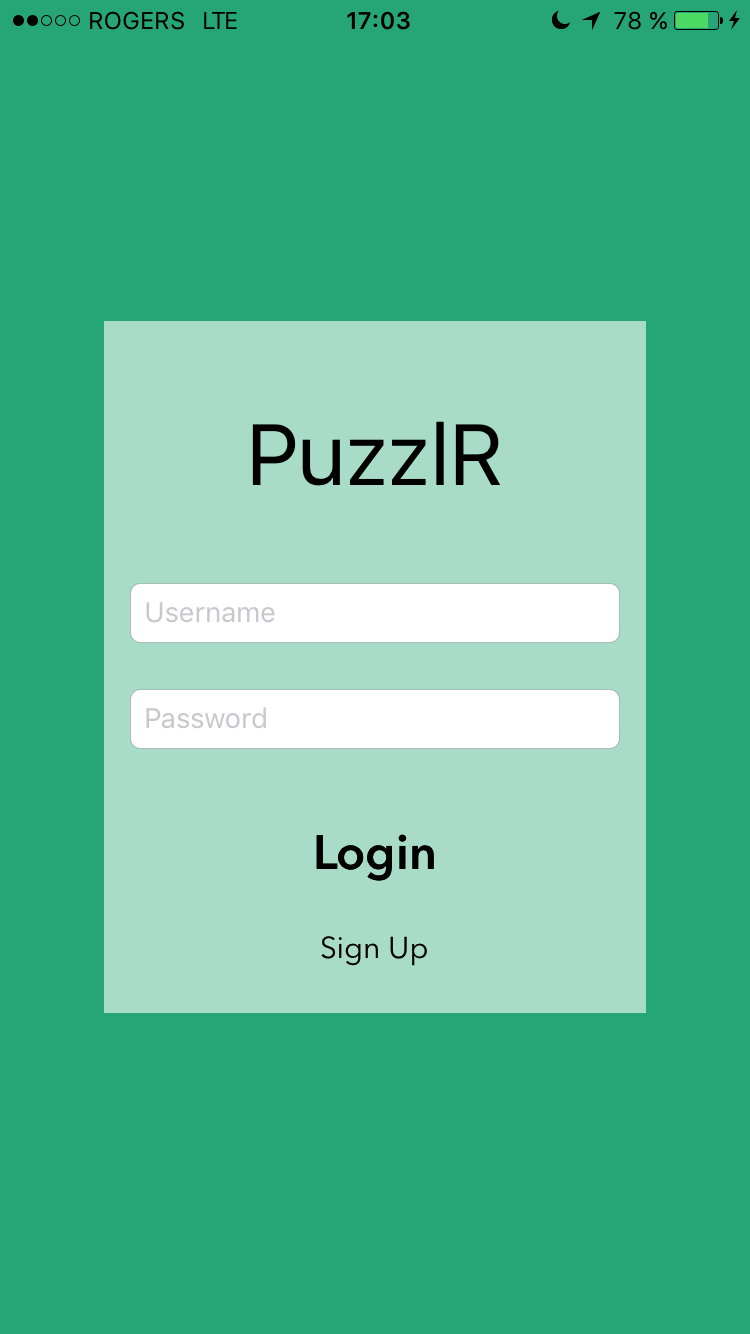
\includegraphics[width=4cm]{images/iOS/login}
	     		 \caption{Login page of Puzzlr iOS}
	   		\end{figure}
	   		When opening the app for the first time, the user is prompted to register. Once he is registered, a keypair is generated and stored securely in the iOS keychain. He can now add contact in the contact menu by writing his friend's username. If the previous friend is registered the app will retrieve his public key and store it in the iOS keychain. The user only have to create a new message, entering his friend's username and adding a photo. His friend will receive the picture instantaneously on his iDevice.
